\section{Design Patterns}
\begin{itemize}
	\item What are Design Patterns
	\begin{itemize}
		\item Descriptions of communicating objects and classes that are customized to \textbf{\underline{solve}} a general design \textbf{\underline{problem}} in a particular \textbf{\underline{context}}
		\item 	Gamma et al. described 23 design patterns divided into three categories:
		\begin{enumerate}
			\item Creational patterns
			\item Structural patterns
			\item Behavioral patterns
		\end{enumerate}
	\end{itemize}

	\item Creational Patterns
	\begin{itemize}
		\item Concern the process of object creation
		\item Six creational patterns
		\vspace{-\itemsep}
		\begin{enumerate}
		\begin{minipage}[t]{\widthof{Abstract Factory} + 1cm}
%			\begin{enumerate}
				\item Factory Method
				\item Abstract Factory
				\item Singleton
%			\end{enumerate}
		\end{minipage}
		\begin{minipage}[t]{\widthof{Object pool} + 1cm}
%			\begin{enumerate}
				\setcounter{enumi}{3}
				\item Prototype
				\item Builder
				\item Object Pool
%			\end{enumerate}
		\end{minipage}
		\end{enumerate}
	\end{itemize}

	\item Structural Patterns
	\begin{itemize}
		\item Deal with the composition of classes or objects
		\item Seven structural patterns
		\vspace{-\itemsep}
		\begin{enumerate}
		\begin{minipage}[t]{\widthof{Composite} + 1cm}
				\item Adapter
				\item Bridge
				\item Composite
				\item Decorator
		\end{minipage}
		\begin{minipage}[t]{\widthof{Flyweight} + 1cm}
				\setcounter{enumi}{4}
				\item Facade
				\item Flyweight
				\item Proxy
		\end{minipage}
		\end{enumerate}
	\end{itemize}

	\item Behavioral Patterns
	\begin{itemize}
		\item Characterize the ways in which classes or objects interact and distribute responsibility
		\item Ten Behavioral patterns
		\begin{enumerate}
		\begin{minipage}[t]{\widthof{Chain of Responsibility} + 1cm}
				\item Chain of Responsibility
				\item Command
				\item Interpreter
				\item Iterator
				\item Mediator
		\end{minipage}
		\begin{minipage}[t]{\widthof{Observer} + 1cm}
				\setcounter{enumi}{5}
				\item Memento
				\item Observer
				\item State
				\item Strategy
				\item Template
		\end{minipage}
		\end{enumerate}
	\end{itemize}

	\item Singleton (Creational)
	\begin{itemize}
		\item Intent: Ensure a class has only one instance, and provide a global point of access to it\\
		\begin{center}
			\begin{tabular}{| l |}
				\hline
				Singleton\\
				\hline
				$ - $instance: Singleton\\
				\hline
				$ - $Singleton()\\
				+getInstance(): Singleton\\
				\ldots\\
				\hline
			\end{tabular}	\textit{	( $ - $ means private, $ + $ means public)}
		\end{center}
	\end{itemize}
	%
	\item Facade (Structural)
	\begin{itemize}
		\item Intent: Hide complexities and provide a unified interface to a set of interfaces in a subsystem\\[-10pt]
		\begin{center}
			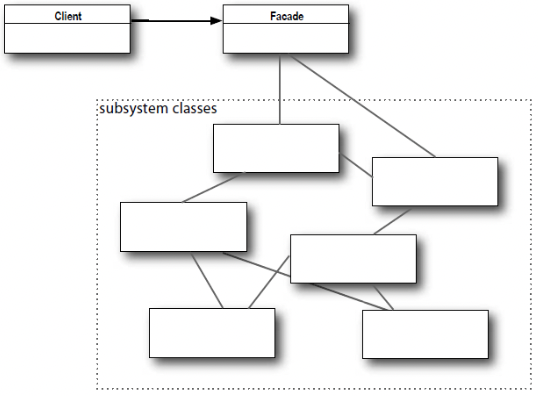
\includegraphics[scale=0.8]{Facad.png}
		\end{center}
	\end{itemize}
%	\newpage
	\item Adapter (Structural)
	\begin{itemize}
		\item Intent: Let classes work together that couldn't otherwise because of incompatible interfaces\\[-10pt]
%		\begin{center}
%			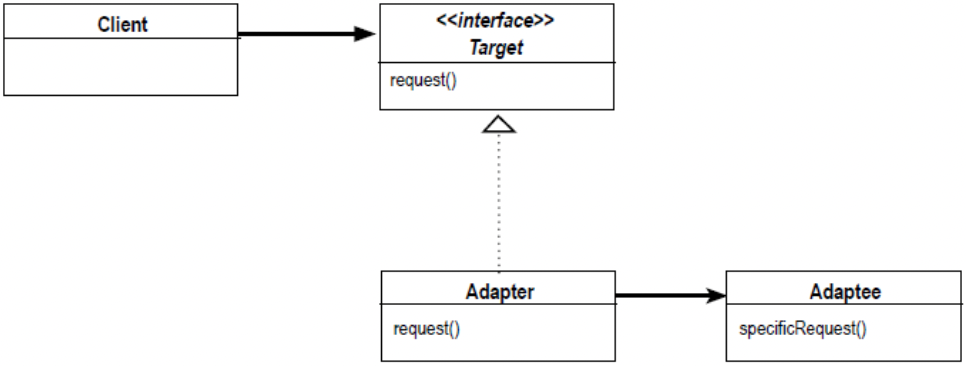
\includegraphics[scale=0.7]{Adapter.png}
%		\end{center}
		\begin{figure}[h!]
			\centering
			\scalebox{0.8}{\begin{tikzpicture}
				\node[type] (target) {
					\textbf{$ \langle\langle $Interface$ \rangle\rangle $} \\
					\Verb|Target|};

				\node[method] (request) [below=0pt of target] {request()};

				\node[type] (client) [left=of target] {\Verb|Client|};
				\node[method] () [below=0pt of client] {};

				\draw[very thick, -Latex] (client.east) -- (target.west);

				\node[type] (adapter) [below=2cm of target] {\Verb|Adapter|};
				\node[method] () [below=0pt of adapter] {request()};

				\node[type, minimum width=3.2cm] (adaptee) [right=of adapter] {\Verb|Adaptee|};
				\node[method, minimum width=3.2cm, text width=2.9cm] () [below=0pt of adaptee] {specificRequest()};

				\draw[densely dotted,-{Triangle[open, width=2.5mm, scale=1.3]}, shorten >= 1pt, thick] (adapter.north) -- (request.south);
				\draw[very thick, -Latex] (adapter.east) -- (adaptee.west);
			\end{tikzpicture}}
		\end{figure}
	\end{itemize}

	\item Observer (Behavioral)
	\begin{itemize}
		\item Intent: Define a one-to-many dependency between objects so that when one object changes state, all its dependents are notified and updated automatically\\[-10pt]
%		\begin{center}
%			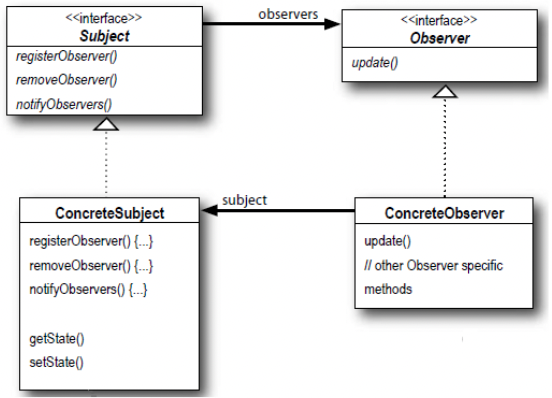
\includegraphics[scale=0.9]{Observer.png}
%		\end{center}
		\begin{figure}[h!]
			\centering
			\scalebox{0.8}{\begin{tikzpicture}
				\node[type, text width=1.2in] (subject) {\textbf{$ \langle\langle $Interface$ \rangle\rangle $} \\ \Verb|Subject|};
				\node[method, text width=1.2in, align=left] (stype) [below=0pt of subject] {\textit{registerObserver()} \\ \textit{removeObserver()} \\ \textit{notifyObservers()}};

				\node[type, text width=1.2in] (observer) [right=1.2in of subject] {\textbf{$ \langle\langle $Interface$ \rangle\rangle $} \\ \Verb|Observer|};
				\node[method, text width=1.2in, align=left] (otype) [below=0pt of observer] {\textit{update()}};

				\node[type, text width=1.6in] (consubject) [below=of stype]{\Verb|ConcreteSubject|};
				\node[method, text width=1.6in, align=left] (ctype) [below=0pt of consubject] {{registerObserver() \{...\}} \\ {removeObserver() \{...\}} \\ {notifyObservers() \{...\}} \\ \phantom{Empty space} \\ getState() \\ setState()};

				\node[type, text width=1.6in] (conobserver) [right=0.8in of consubject] {\Verb|ConcreteObserver|};
				\node[method, text width=1.6in] (cotype) [below=0pt of conobserver] {update() \\ // other Observer Specific \\ Methods};

				\draw[-Latex, thick] (subject) -- (observer) node[above, pos=0.65] () {{\small observers}};
				\draw[-Latex, thick] (conobserver) -- (consubject) node[above, pos=0.65] () {{\small subject}};
				\draw[densely dotted,-{Triangle[open, width=2.5mm, scale=1.3]}, thick] (consubject) -- (stype);
				\draw[densely dotted,-{Triangle[open, width=2.5mm, scale=1.3]}, thick] (conobserver) -- (otype);
			\end{tikzpicture}}
		\end{figure}
	\end{itemize}
	%	\newpage
	\item Strategy (Behavioral)
	\begin{itemize}
		\item Intent: Define a family of algorithms, encapsulate each one, and make them interchangeable\\
%		\begin{center}
%			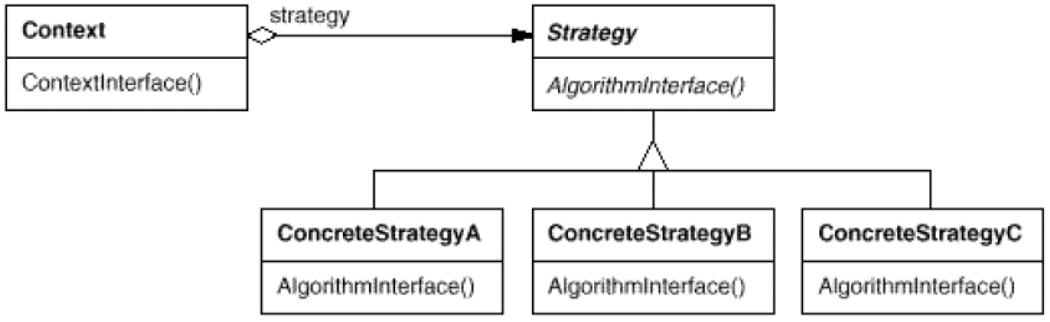
\includegraphics[scale=0.8]{Strategy.png}
%		\end{center}
			\scalebox{0.8}{\begin{tikzpicture}
				\node[type, align=left, text width=1.5in] (strategy) {\textit{\textbf{Strategy}}};
				\node[method, text width=1.5in] (stratmeth) [below=0pt of strategy] {\textit{AlgorithmInterface()}};

				\node[type, text width=1.5in] (stratb) [below=of stratmeth] {\textbf{ConcreteStrategyB}};
				\node[method, text width=1.5in] () [below=0pt of stratb] {AlgorithmInterface()};

				\node[type, text width=1.5in] (stratc) [right=of stratb] {\textbf{ConcreteStrategyC}};
				\node[method, text width=1.5in] () [below=0pt of stratc] {AlgorithmInterface()};

				\node[type, text width=1.5in] (strata) [left=of stratb] {\textbf{ConcreteStrategyA}};
				\node[method, text width=1.5in] () [below=0pt of strata] {AlgorithmInterface()};

				\node[type, text width=1.5in] (context) [left=2.3in of strategy] {\textbf{Context}};
				\node[method, text width=1.5in] () [below=0pt of context] {ContextInterface()};

				\draw[-{Triangle[open, length=1.5mm, scale=2]}] (stratb.north) -- ([yshift=19.5pt]stratb.north);
				\draw (strata.north) |- ([yshift=11pt]stratb.north) -| (stratc.north);
				\draw ([yshift=19pt]stratb.north) -- (stratmeth);

				\draw[-{Diamond[open, scale=2]}] (strategy) -- (context) node[above, pos=0.8] () {{\small strategy}};
			\end{tikzpicture}}
	\end{itemize}
\end{itemize}
